% !TeX spellcheck = french
\documentclass[12pt]{report}
\usepackage{longtable}
\usepackage[table,xcdraw]{xcolor}
\usepackage[utf8]{inputenc}
\usepackage[T1]{fontenc}
\usepackage[francais]{babel}
\usepackage{fixltx2e}
\usepackage{charter}
\usepackage{amsmath}
\usepackage{float}
\usepackage{wrapfig}
\usepackage{graphicx}
\usepackage{soul}
\usepackage[colorlinks=true, linkcolor=blue]{hyperref}
\usepackage[a4paper, width=150mm, top=25mm, bottom=25mm]{geometry}
\usepackage{parskip}
\usepackage{enumitem}
\usepackage[final]{pdfpages}
\usepackage[linguistics]{forest}
%\usepackage{titlesec}
\usepackage{listings}
\usepackage[final]{pdfpages}
\usepackage[font=small,labelfont=bf]{caption} % Required for specifying captions to tables and figures
\setlist[itemize]{label=\textbullet}
\usepackage[linesnumbered,algoruled,french,onelanguage]{algorithm2e}
\usepackage{url}
\usepackage{amsmath}
\usepackage{algorithmicx}
\usepackage{xcolor}
\usepackage{multirow}
\usepackage[noend]{algpseudocode}
\usepackage{tabularx}  % for tabularx
% to make cells in table have decent spacing
\usepackage{array}
\newcolumntype{L}[1]{>{\raggedright\let\newline\\\arraybackslash\hspace{0pt}}m{#1}}
\newcolumntype{C}[1]{>{\centering\let\newline\\\arraybackslash\hspace{0pt}}m{#1}}
\newcolumntype{R}[1]{>{\raggedleft\let\newline\\\arraybackslash\hspace{0pt}}m{#1}}

\lstset{
	language=Python,                   % choix du langage (de programmation).
	keywordstyle=\color{blue},      % choix de la couleur des mots clés.
	stringstyle=\color{red},        % choix de la couleur des string.
	commentstyle=\color{green},     % choix de la couleur des commentaire.
	basicstyle=\normalsize,     % taille de la police du code
	% numbers=left,                   % placer le numéro de chaque ligne à gauche (on peut choisir à droite, ou ne pas mettre cette option pour aucun numéro de ligne).
	numberstyle=\normalsize,        % taille de la police des numéros.
	numbersep=0pt,                  % distance entre le code et sa numérotation.
	showstringspaces=false,         % pour ne pas afficher les espaces comme des caractères .
	breaklines=true,                % couper la ligne si la ligne du code est trop longue.
}
\def \hfillx {\hspace*{-\textwidth} \hfill}


\begin{document}

\includepdf[pages=1]{Page_garde.pdf} 
\tableofcontents

\pagenumbering{arabic}
\newpage
\chapter{Introduction : }
\section{Problématique : }
\paragraph{}
Dans ce TP, nous allons tenter d'implémenter et de comparer plusieurs méthodes aveugles, dites aussi \textbf{à base d'espace d'états}, Pour la résolution du problème de satisfiabilité, plus communément appelé \textbf{Problème SAT}, Ce travail est aussi une application directe des différentes méthodes vues durant le premier semestre en ce qui concerne la \textbf{Résolution de problèmes}, mais aussi la \textbf{Complexité des algorithmes et les structures de données}.
\section{Définitions}
\paragraph{}
Avant de rentrer dans les détails de la résolution du problème, nous devons d'abord définir ce qu'est le problème SAT, ainsi que les différentes méthodes utilisées pour sa résolution dans ce TP.
\subsection{Problème SAT}
\paragraph{}
Dans le domaine de l'informatique et de la logique, le problème de satisfiablité (\textbf{SAT}), est un problème de décision ou il s'agit d'assigner des valeurs de vérité à des literaux\footnote{Une variables logique ou bien sa négation} tel qu'un ensembles de clauses en forme normale conjonctives FNC\footnote{Une conjonction de disjonction de litéraux} préalablement défini soit satisfiable, en d'autres termes, que toutes les clauses soient vraies pour les mêmes valeurs de vérité de leurs literaux, ce problème est le premier à avoir été démontré comme étant \textbf{NP-Complet}, et cela par \href{https://en.wikipedia.org/wiki/Stephen_Cook}{Stephen Cook} dans \cite{cook}, et qui a donc posé les fondements de l'informathique théoriques et de la théorie de la complexité.
\newpage
\subsection{Stratégie de recherche dans l'espace des états}
En cosidérant l'espace de recherche comme étant une arborescence, dont les noeuds sont les differents états du problème, nous pouvons classer les différentes stratégies de recherches en deux grandes catégories :
\subsection{Stratégie de rercherche aveugle}
\paragraph{}Cette catégories englobe les stratégies ou il est question de passer par toutes les solutions et les tester une à une, dans ce TP nous nous intéresserons plus particulièrement aux algortihmes/methodes suivant(es) :  
\subsubsection{Par prodonfeur d'abord (DFS)}
\paragraph{}
L'algorithme de parcours en profondeur d'abord consiste a visité un noeud de départ (souvent appelé \textbf{racine}), puis ensuite visite le premier sommet voisin(ou \textbf{successeur}) jusqu'à ce qu'une profondeur limite soit atteinte ou bien qu'il n'y ait plus de voisin à developper, une variante de cet algorithme utilise deux ensemble \textbf{Open} et \textbf{Closed} qui représentent réspectivement l'ensemble des noeuds du graphe qui n'ont pas encore étés developpés et ceux déjà développés, cet ajout permet à l'algorithme d'éviter de boucler indéfiniment sur un ensemble de noeuds.
\subsubsection{En Largeur d'abord (BFS)}
\paragraph{}
Cet algorithme diffère de son prédecesseur par le fait qu'il visite tous les voisins(\textbf{successeurs}) d'un noeud avant de passer au noeud suivant, ce qui revient à gérer l'ajout et la suppression de l'ensemble Open comme une file, donc en mode \textbf{FIFO} (En supposant bien sûr qu'on dispose des deux ensembles open et closed), cet approche permet de sauvegarder tous les noeuds précèdemment visité durant la recherche, ce qui peut causer un débordement de la mémoire lors de l'exécution sur machine(Ce point sera rediscuté dans \ref{BreadthIssue} page \pageref{BreadthIssue} et \ref{BreadthIssueExperience} page \pageref{BreadthIssueExperience} et \ref{BreadthIssueCompare} page \pageref{BreadthIssueCompare})

\subsubsection{Par coût uniforme}
\paragraph{}
Le principe est simple, au fur et à mesur que l'algorithme avance et développe des noeuds, il garde en mémoire le coût\footnote[1]{Fonction retournant le cout pour passer du noeud de départ(la racine) au noeud courant}, le noeud qui sera ensuite choisi sera celui dont le coût accumulé est le plus bas, assurant ainsi de toujours choisir le chemin le plus optimal, si le coût pour passer d'un noeud à n'importe quel autre de ses voisins est le même quelque soit le neoud, l'algorithme est alors équivalent à celui de la recherche en largeur d'abord

\subsection{Stratégie de rercherche guidée}
Cette catégorie englobe quant à elle les stratégies ou il est question de parcourir une plus petite partie de l'espace de recherche dans l'espoir de trouver la solution optimal en un temps plus réduit, les algortihmes sont les suivants : 
\subsubsection{Recherche gloutonne (Greedy algorithm)}
\paragraph{}
Cet algorithme est basé sur la notion d'heuristique\footnote[1]{Une fonction d'éstimation de la distance séparant le noeud courant au but }, au lieu de parcourir de façon "naïve" l'ensemble des noeuds dans l'espace de recherche, il choisit a chaque itérration sur l'ensemble \textbf{open} le noeud le plus \textbf{prometteur} en terme de distance par rapport au but recherché.
\subsubsection{Algorithme A*}
\paragraph{}
Contrairement aux précedents algorithmes de recherche qui effectuaient une recherche de façon "naîve", l'algorithme \textbf{A* }propose une vision un peu nouvelle, il utilise la notion de coût et celle d'heuristique, la fonction d'évaluation $f$ est donc définie comme étant la somme de deux fonctions $g$ et $h$ ou : \\
	\begin{itemize}
		\item $g$ est la fonction  qui retourne le cout d'un noeud $n$
		\item $h$ est la fonction  qui estime le cout d'un noeud $n$ vers le but
	\end{itemize} 
Le principe de l'algorithme est donc de prendre le noeud dans \textbf{open} qui possède la valeur minimal de $f$, assurant ainsi de trouver le chemin optimal \textbf{ssi.} l'heuristique $h$ choisie est admissible\footnote[2]{Ne surestime jamais le coût réel pour atteindre le but, elle est \textbf{optimiste}}


\newpage
\chapter{Implémentation}
\section{Structures de données}
\paragraph{}
La stratégie de recherche avec graphe requiert une représentation des entrées du problème, des états construisant une solution potentielle à ce dernier ainsi que le développement de ces états.
\subsection{Représentation du problème SAT}
\paragraph{}
Une instance du problème SAT peut être considérée comme un ensemble de clauses, chacune de ces clauses est une disjonction de littéraux. Dans ce rapport Nous proposons deux structures différentes pour les représenter que nous comparerons par la suite.
\subsubsection{Représentation matricielle}
\paragraph{}
Une première représentation serait d‘associer à chaque clause de l’instance un tableau de taille égale au nombre de variables logiques utilisés dont la i\up{ième}  case aura la valeur 1 si la variable \textit{i} est présente dans la clause, -1 si sa négation est présente, 0 sinon. Ainsi en représentant toutes les clauses on obtient une matrice dont chaque ligne est associée à une clause.\\
L’exemple suivant montre une instance du problème SAT et sa représentation matricielle:
\begin{flalign*}
x_{1} \lor \neg x_{2} \lor x_{5} \\
\neg x_{2} \lor x_{4} \lor x_{5} \\
\neg x_{1} \lor x_{2} \lor \neg x_{3}
\end{flalign*}
Ces clauses vont être représentée comme suit:
\begin{center}
	\parbox{.2\textwidth}{
		\begin{tabular}{|c|c|c|c|c|}
			\hline
			1&-1&0&0&1\\
			\hline
			0&-1&0&1&1\\
			\hline
			-1&1&1&0&0\\
			\hline
		\end{tabular}}
\end{center}
\newpage

\subsubsection{Représentation par \textit{Bitset}}
\paragraph{}
On pourrait aussi aborder la représentation du point de vu littéral, c’est à dire associer à chaque littéral les clauses dans lesquels il est présent. Pour cela un tableau de bits appelé \textit{Bitset} pourrait être utilisé où chaque bit \textit{i} aurait la valeur 1 si la i\up{ième} clause contient le littéral, la valeur 0 sinon. On obtient donc un tableau de taille 2 fois le nombre de variables utilisés dont les entrés représentent les \textit{Bitsets} des littéraux.\\
Pour le même exemple vu précédemment on obtient les \textit{Bitsets} suivants:\\\\
	\begin{minipage}{0.5\textwidth}
		\centering
		\begin{tabular}{|c | c| c| c|}
			\hline
			$x_{1}$& 1 & 0 & 0 \\\hline
			$x_{2}$& 0 & 0 & 0 \\\hline
			$x_{3}$& 0 & 0 & 0 \\\hline
			$x_{4}$& 0 & 1 & 0 \\\hline
			$x_{5}$& 1 & 1 & 0 \\\hline
		\end{tabular}
	\end{minipage}
	\hfillx
	\begin{minipage}{0.5\textwidth}
		\centering
		\begin{tabular}{|c | c| c| c|}
			\hline
			$\neg x_{1}$& 0 & 0 & 1 \\\hline
			$\neg x_{2}$& 1 & 1 & 0 \\\hline
			$\neg x_{3}$& 0 & 0 & 1 \\\hline
			$\neg x_{4}$& 0 & 0 & 0 \\\hline
			$\neg x_{5}$& 0 & 0 & 0 \\\hline
		\end{tabular}
	\end{minipage}

\subsection{Représentation des états}
\paragraph{}
Une solution à une instance du problème SAT se réduit à l’assignation des valeurs de vérités aux variables logiques de cette instance. On peut considérer un état dans l’espace de recherche comme étant le choix de la valeur de vérité d’une des variables logiques, on obtient après une succession de choix une solution au problème qui peut être positive si les valeurs assignés sont consistante avec les clauses de l’instance, négative sinon. Nous allons représenter un état avec un noeud qui contient le numéro de la variable choisie, multiplié par -1 pour désigner l’assignation de la valeur $faux$ à la variable, il reste inchangé sinon.\\
\begin{center}
	\begin{forest} [
		[5[$x_{5} \leftarrow vrai$]]
		[-5[$x_{5} \leftarrow faux$]]
		]
	\end{forest}
\end{center}
\newpage
\subsection{Développement des états}
\paragraph{}
A partir de chaque état on peut faire le choix de la valeur de vérité d’une variable logique choisie aléatoirement. Le développement d’un noeud donne deux successeurs, un pour chaque valeur de vérité assignée à la prochaine variable. On obtient après l’exploration de l’espace de recherche un arbre d’états, l’exemple suivant est un arbre associé à une instance SAT contenant trois variables.\\
\begin{center}
	\begin{forest} [
		[2
			[1
				[3]
				[-3]
			]
			[-1
				[3]
				[-3]
			]
		]
		[-2
			[1
				[3]
				[-3]
			]
			[-1
				[3]
				[-3]
			]
		]
		]
	\end{forest}
\end{center}
Une solution est représentée par une branche de l’arbre, par exemple la solution : $x_{1} = vrai$, $x_{2} = faux$, $x_{3} = faux$ est représentée dans l’arbre précédent comme suit:
\begin{center}
	\begin{forest} [
		[2
		[1
		[3]
		[-3]
		]
		[-1
		[3]
		[-3]
		]
		]
		[-2, text=red
		[1, text=red
		[3]
		[-3, text=red]
		]
		[-1
		[3]
		[-3]
		]
		]
		]
	\end{forest}
\end{center}
Pour pouvoir construire une solution à partir de n’importe quel noeud, on doit y sauvegarder l’adresse de son parent, ainsi on peut récupérer les valeurs assignées aux noeuds précédents jusqu’à la racine. L’enregistrement suivant représente un noeud de l’arbre:

\begin{lstlisting}
struct {
int valeur; 
struct noeud* parent;
} noeud;
\end{lstlisting}

\paragraph{Remarque1:}\label{BreadthIssue} Un inconvénient que nous avons déjà cité de la recherche en largeur d’abord était la saturation rapide de la mémoire, cela est dû au fait de garder tous les noeuds dans la mémoire. Ce problème est évité dans la recherche en profondeur d’abord car dès l’évaluation d’un noeud se trouvant dans la profondeur maximale, ce dernier est supprimé de la mémoire. notons que la structure du noeud déjà présenté ne contient pas les adresses de ses successeurs, ceci nous permet d’éviter de garder tous l’arbre d’états dans la mémoire mais juste les branche susceptible d’être évaluée par la suite.\\~\\
\paragraph{Remarque2:} Dans la deuxième représentation du problème SAT, une optimisation serait d’ajouter un $Bitset$ dans la structure du noeud et y garder les clauses qu’il satisfait ainsi que celles de ses parents, celui là peut être obtenu en appliquant l’opération OU logique sur le $Bitset$ du noeud parent et celui du littéral choisi.\\
\begin{center}
	\begin{minipage}{0.5\textwidth}
		\centering
		\begin{tabular}{|c | c| c| c|c|}
			\hline
			$Bitset$ du parent& 1 & 0 & 1 & 1 \\\hline
		\end{tabular}
	\end{minipage}
	\\~\\
	OR
	\\~\\
	\begin{minipage}{0.5\textwidth}
		\centering
		\begin{tabular}{|c | c| c| c|c|}
			\hline
			$Bitset$ du littéral& 1 & 0 & 0 & 1\\\hline
		\end{tabular}
	\end{minipage}
	\begin{center}

		$\downarrow$
		\\~\\
		\begin{tabular}{|c | c| c| c|c|}
			\hline
			$Bitset$ du noeud& 1 & 0 & 1 & 1\\\hline
		\end{tabular}
	\end{center}
\end{center}

\section{Conception et pseudo-code}
\paragraph{}
Dans cette partie nous allons présenter l’implémentation des algorithmes de recherche avec graphe, un algorithme générique qui englobe les différente méthodes est présenté si dessous:

\begin{algorithm}
	\SetAlgoLined
	\KwResult{retourne la solution ou échec}
	$open \gets \textbf{état initial}$\;
	initialiser l'ensemble $closed$ à \textbf{vide}\;
	\While{$\neg$\textbf{vide} $open$}{
		$noeud \gets$ \textbf{choisir\_noeud($open$)}\;
		\If{\textbf{noeud\_but}($noeud$)}{
			\Return \textbf{solution}($noeud$)\;
		}
		\textbf{ajouter}($noeud$,$closed$)\;
		$successeurs \gets$ \textbf{developper}($noeud$) \;
		inserer les $sueccesseurs$ qui n'appartiennent pas à $closed$ dans $open$ 
	}
	\Return echec\;
\caption{Algorithme de recherche avec graphe}
\end{algorithm}
\paragraph{}
La différence entre les algorithmes de recherche réside dans la manière dont on sélectionne le noeud à évaluer, ligne 4 dans l’algorithme si dessus, ainsi que l’estimation du coût et de l’heuristique, s’ils existent, avant l’insertion, ligne 10.\\
\paragraph{}
En se basant sur cette algorithme nous avons implémenter une procédure de recherche générique prenant en paramètre un type de gestion de liste, un estimateur de coût et d’heuristique et les entrés de l’instance SAT afin d’évaluer les noeuds.
\subsection{Gestion de la liste open}
\paragraph{}
Les méthodes partagent quasiment le même pseudo code, à l'excéption de la façon dont la liste \textbf{open} est géré, en insertion et en supression.
\subsubsection{Profondeur d'abord}
\paragraph{}
La recherche en profondeur d’abord consiste à choisir le noeud avec la profondeur la plus élevé de l’arbre, ceci reviens à sélectionner l’élément le plus récemment inséré dans la liste open, c’est à dire, la gérer avec une politique LIFO.\\
Insertion d'un noeud:\\
\begin{minipage}{0.5\textwidth}
	\centering
	\begin{tabular}{|c |}
		\hline
		 3 \\
		\hline
	\end{tabular}
\end{minipage}
\hfillx
$\rightarrow$
\begin{minipage}{0.5\textwidth}
	\centering
	\begin{tabular}{|c | c| c| c|}
		\hline
		{\color{red}3} & -3 & -2 & -1 \\\hline
	\end{tabular}
\end{minipage}

Sélection d'un noeud:\\
\begin{minipage}{0.5\textwidth}
	\centering
	\begin{tabular}{|c |}
		\hline
		{\color{red}3} \\
		\hline
	\end{tabular}
\end{minipage}
\hfillx
$\leftarrow$
\begin{minipage}{0.5\textwidth}
	\centering
	\begin{tabular}{| c| c| c|}
		\hline
		-3 & -2 & -1 \\\hline
	\end{tabular}
\end{minipage}


\subsubsection{Largeur d'abord}
\paragraph{}
Contrairement à la recherche en profondeur d’abord, les noeuds sont visités de tel sorte à parcourir l’arbre niveau par niveau, cela peut être réalisé par la sélection du noeud le moins récemment insérer dans open, d’où une gestion LIFO de la liste.\\
Insertion d'un noeud:\\
\begin{minipage}{0.5\textwidth}
	\centering
	\begin{tabular}{|c |}
		\hline
		3 \\
		\hline
	\end{tabular}
\end{minipage}
\hfillx
$\rightarrow$
\begin{minipage}{0.5\textwidth}
	\centering
	\begin{tabular}{|c | c| c| c|}
		\hline
		{\color{red}3} & -3 & -2 & -1 \\\hline
	\end{tabular}
\end{minipage}

Sélection d'un noeud:\\
\begin{minipage}{0.5\textwidth}
	\centering
	\begin{tabular}{|c |}
		\hline
		{\color{red}-1} \\
		\hline
	\end{tabular}
\end{minipage}
\hfillx
$\leftarrow$
\begin{minipage}{0.5\textwidth}
	\centering
	\begin{tabular}{| c| c| c|}
		\hline
		3 & -3 & -2  \\\hline
	\end{tabular}
\end{minipage}

\subsubsection{Recherche En se basant sur une fonction d'évaluation}
\paragraph{}
Dans ce type de recherche, la sélection d’un noeud se fait sur la base d’une fonction d’évaluation. Le noeud sélectionné est celui avec la valeur minimale (resp. maximale) de la fonction d’évaluation. Nous utilisons ce type de gestion afin d’implémenter les algorithmes: recherche à coût uniforme, recherche gloutonne et l’algorithme A*.\\
Nous avons implémenter ce type de gestion avec deux structures différentes que nous comparerons dans la suite de ce rapport.
\paragraph{Liste triée}
Les noeuds sont triés dans une liste selon leur valeur estimé par la fonction d’évaluation. Le premier noeud est toujours sélectionner, l’insertion par contre se fait de tel sorte à garder la liste triée en ordre croissant (resp. décroissant).\\
Insertion d'un noeud:\\
\begin{minipage}{0.5\textwidth}
	\centering
	\begin{tabular}{|c |c|}
		\hline
		3 & $f_{3}=5$\\
		\hline
	\end{tabular}
\end{minipage}
\hfillx
$\rightarrow$
\begin{minipage}{0.5\textwidth}
	\centering
	\begin{tabular}{| c| c|c | c| c| c|}
		\hline
		 -3& $f_{-3}=2$ & {\color{red}3}& {\color{red}$f_{3}=5$} & -1& $f_{-1}=8$ \\\hline
	\end{tabular}
\end{minipage}

Sélection d'un noeud:\\
\begin{minipage}{0.5\textwidth}
	\centering
	\begin{tabular}{|c |c|}
		\hline
		{\color{red}-3} & {\color{red}$f_{-3}=2$}\\
		\hline
	\end{tabular}
\end{minipage}
\hfillx
$\leftarrow$
\begin{minipage}{0.5\textwidth}
	\centering
	\begin{tabular}{|c | c| c| c|}
		\hline
		3& $f_{3}=5$ & -1& $f_{-1}=8$ \\\hline
	\end{tabular}
\end{minipage}\\~\\
Complexité de l’insertion : $o(n)$.\\
Complexité de la sélection : $o(1)$.\\


\paragraph{Tas}
Les noeuds sont organisé dans une structure de tas\footnote{un tas est un arbre équilibré dont chaque noeud a une clé supérieur (resp. Inférieur) à celle de ses fils}. La racine du tas est sélectionner pour l’évaluation, tandis que l’insertion se fait par entassement du nouveau élément. Les deux opérations se font en $o(log(n))$.

\subsection{Fonction d'évaluation}
\paragraph{}
La fonction d’évaluation f d’un noeud n est généralement définit à l’aide de deux autres fonctions g et h. La première désigne le coût nécessaire pour atteindre le noeud n à partir de la racine, tandis que la deuxième est une heuristique qui estime le coût restant avant d’arriver au but.
\subsubsection{Recherche gloutonne}
\paragraph{}
La fonction d’évaluation dans ce cas f est égale à h, on se contente de la valeur estimé par l’heuristique pour décider le prochain noeud à développer. Une heuristique pour le problème SAT qui peut mesurer la distance des noeuds par rapport au noeud but serait de calculer le nombre de clauses pas encore satisfaites, le noeud avec la valeur minimale de cette heuristique est le noeud qui satisfait le plus de clauses et donc le plus proche de satisfaire toutes les clauses.
\subsubsection{Recherche à coût uniforme}
\paragraph{}
Contrairement à la recherche gloutonne, la recherche à coût uniforme n’utilise que la fonction g, permettant ainsi de développer le noeud le plus proche de la racine en terme de coût. Cependant trouver une fonction d’estimation du coût pour le problème SAT s’avère délicat comme on ne peut pas vraiment déterminer une distance entre un noeud et la racine. Ceci dit, une fonction de coût qui calcule le nombre de clauses devant être satisfaite par un noeud mais qui sont déjà satisfaite par ses parents peut être utilisé. Cela représente la perte d’une branche contenant des littéraux qui satisfont les même clauses de l’instance SAT, plus le coût est élevé, moins les chances que cette branche nous mène au but.

\begin{minipage}{0.5\textwidth}
	\centering
	\begin{tabular}{|c | c| c| c|c|}
		\hline
		$Bitset$ du parent& {\color{red}1} & 0 & 0 & 1 \\\hline
	\end{tabular}
\end{minipage}
$\rightarrow$
\begin{minipage}{0.5\textwidth}
	\centering
	\begin{tabular}{|c | c| c| c|c|}
		\hline
		$Bitset$ du littéral& {\color{red}1} & 1 & 0 & 0\\\hline
	\end{tabular}
\end{minipage}
\begin{center}
	$cout = 1$
\end{center}

\subsubsection{Algorithme A*}
\paragraph{}
L’algorithme A* combine les deux fonctions g et h citées précédemment afin d’évaluer les noeuds en prenant en considération le nombre de clauses déjà satisfaites ainsi que le coût de la branche dans laquelle il se trouve.
\subsection{Évaluateur SAT}
\paragraph{}
Dans cette partie nous présentons deux méthodes d’évaluation du noeud but basé sur les deux structures représentatives des instances SAT citées précédemment.
\subsubsection{Évaluation par matrice}
\paragraph{}
La première méthode consiste à parcourir la matrice des clauses et chercher pour chaque clause si un de ses littéraux a été évalué vrai par les noeuds de la solution. Si dessous l’algorithme correspondant.\\
\begin{algorithm}
	\SetAlgoLined
	\KwResult{retourne un booléen: vrai si la solution est positive, faux sinon}
	\textbf{entré}: $solution$\;
	\For{$clause \in$ $matrice$}{
		$satC\gets faux$ \;
		\For{$noeud \in$ $solution$ et $\neg satC$}{
			\If{$clause[\textbf{abs}(noeud.valeur)]\times$ $noeud.valeur$ > 0}
			{
				$satC\gets vrai$\;
			}
		}
		\If{$satC$}{
			$cpt \gets$ $cpt + 1$\;	
		}
		
	}
	\If{$cpt = \textbf{taille}(matrice)$}
	{
		\Return $vrai$\;
	}
	\Return $faux$\;
	\caption{Algorithme d'évaluation par matrice}
\end{algorithm}
\subsubsection{Évaluation par Bitset}
\paragraph{}
Comme vu précédemment, en utilisant la structure Bitset pour représenter l’instance SAT chaque noeud contient un Bitset des clauses satisfaites par sa branche, il suffit donc de calculer le nombre de bits à 1 pour décider si c’est un noeud but ou pas. Nous utilisons pour cela l’algorithme “Hamming Weight” permettant de calculer le nombre de bits à 1 dans un entier en une complexité constante.

\newpage
\chapter{Expérimentations}
\section{Donnés}\label{dataSet}
\paragraph{}Afin de tester notre programme nous avons opté pour l'utilisation de fichiers benchmark qui vont représenter des instances du problème, dorénavant, et pour être plus conforme avec la terminologie di problème, nous utiliserons le terme \textbf{INSTANCE} pour désigner ces dits fichiers.
\paragraph{}
Les instances nous sont présenté sous forme de fichiers au format \textbf{DIMACS}\footnote{Représentation convetionnelle d'une instance du problème SAT}(plus de détails dans \ref{par:dimacs}) et sont disponibles en téléchargement gratuitement et librement sur \cite{Benchmark}, et sont le fruit du travail de nombreux chercheurs dévoués.
\subsection{Format DIMACS}\label{par:dimacs}
Un fichier en format \textbf{DIMACS} est un fichier dont l'extension est \textbf{.cnf}, et est structuré de la manière suivante : \\
\begin{itemize}
	\item Le fichier peut commencer avec des commentaires, un commentaire sur une ligne commence par le caractère \textbf{"c"}
	\item La première ligne du fichier(après les commentaires) doit être structuré de la manière suivante : \textbf{p cnf nbvar nbclause}
	\begin{enumerate}
		\item \textbf{p cnf} pour indiquer que l'instance est en forme normale conjonctive \textbf{FNC}.
		\item \textbf{nbvar} indique le nombre de litéral au total dans l'instance, à noté que chaque literal $x_{i}$ sera représenté par son indice $i$.
		\item \textbf{nbclause} le nombre total de clause présentes dans l'instance.
	\end{enumerate}
	\item chaque ligne représente une conjonction de litéraux $(x_{i} \vert \lnot x_{i})$ indentifiés par un numero $i$, séparés par un blanc, et le 0 à la fin dénote la fin d'une ligne.
\end{itemize}
\subsection{Example}
c\\
c Un commentaire\\
c\\
c \\
p cnf 5 3\\
1 -5 4 0\\
-1 5 3 4 0\\
-3 -4 0\\
\newpage
\subsection{Type d'instances}
Dans \cite{Benchmark} nous avons à notre disposition deux types d'instances pour chaque taille du problème : \\
\begin{itemize}
	\item Un ensemble d'instances satisfiable dans un fichier dénommé UF\textbf{XX}-\textbf{YY},\\avec \textbf{XX} = nombre de litéraux et \textbf{YY} = nombre de clauses
\end{itemize}
\section{Environement de travail}
\subsection{Machines}
\paragraph{}
Pour les tests nous avons utilisé deux machines pour chaques groupes d'instances, autrement dit une machine pour éffecutuer les tests sur un ensembles d'instances satisfiables \textbf{UF75-325}\cite{Benchmark} et une autre sur les instances contradictoires(non satisfiables) \textbf{UUF75-325}\cite{Benchmark}, les caractéristiques de chaques machines sont données dans les figures \ref{fig:machineA} et \ref{fig:machineB} suivantes : 
\begin{figure}[H]
	\centering
	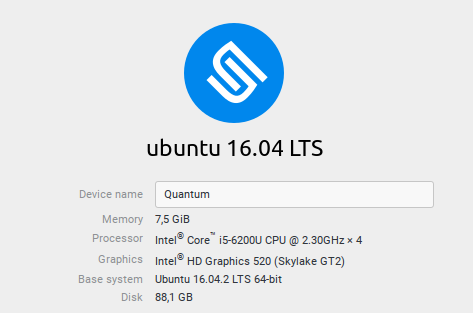
\includegraphics[scale=0.75]{images/machineWISS.png}
	\caption{Machine \textbf{A} pour les instances contradictoires}
	\label{fig:machineA}
\end{figure}
\begin{figure}[H]
	\centering
	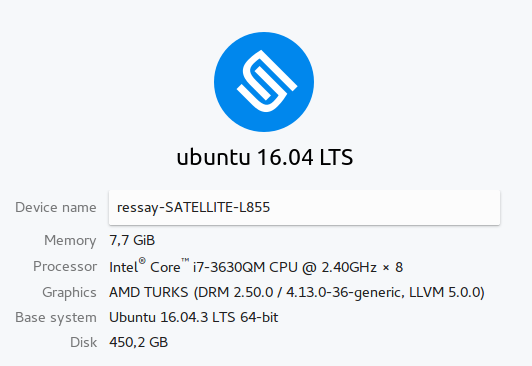
\includegraphics[scale=0.665]{images/machineYASSER.png}
	\caption{Machine \textbf{B} pour les instances satisfiables}
	\label{fig:machineB}
\end{figure}
\newpage
\subsection{Outils utilisés}
\subsubsection{Langage de programmation : }
\paragraph{}

\subsubsection{IDE : }
\paragraph{}
\paragraph{IntelliJ Idea} L'environement de dévelopement choisit est \href{URL}{IntelliJ IDEA}, spécialement dédié au développement en utilisant le langage \href{URL}{JAVA}, il est proposé par l'entreprise \href{https://www.jetbrains.com}{JetBrains} il est caractérisé par sa forte simplicité d'utilisation et les nombreuse plugins et extentions qui lui sont dédiées.

\section{Résultats}\label{tests}
\paragraph{}
\section{Statistiques}
\paragraph{}
\section{Comparaison entres les quatres méthodes}
\paragraph{}
\newpage
\chapter{Conclusion}

\listoffigures
\listoftables
\bibliographystyle{unsrt}
\bibliography{biblio.bib}
\end{document}}